\section{Background and Scope}
\label{sec:background}

\paragraph{E-graphs and equality saturation.}
An e-graph compactly records expressions that have been shown equal under a
chosen set of equations. An \emph{e-node} stores an operator and references to
its child \emph{e-classes}; an e-class groups alternative expressions already
known to be equal. Thus a child reference can stand for several expressions,
and shared subexpressions need not be copied~\cite{ogEgraphs1,egraphsOG,egg}.

For instance, assume an arithmetic language in which $x\times 2=x+x$ is a valid
equation. Let $c_a=\{a\}$ and $c_2=\{2\}$ be singleton e-classes.
The term $a\times 2$ is represented by the e-node
$\times(c_a,c_2)$. Applying the equation does not replace this node:
it adds $+(c_a,c_a)$ and places both alternatives in one e-class,
$$
c=\{\times(c_a,c_2),\; +(c_a,c_a)\}.
$$
A parent e-node $g(c)$ therefore represents both $g(a\times 2)$ and
$g(a+a)$ while sharing their common subterms, as shown in Figure~\ref{fig:typed-slotted-egraphs}(a). 
% Preamble: \usepackage{graphicx,amsmath,amssymb}
% Place typed-slotted-egraphs.pdf beside the main LaTeX source.
\begin{figure}[t]
  \centering
  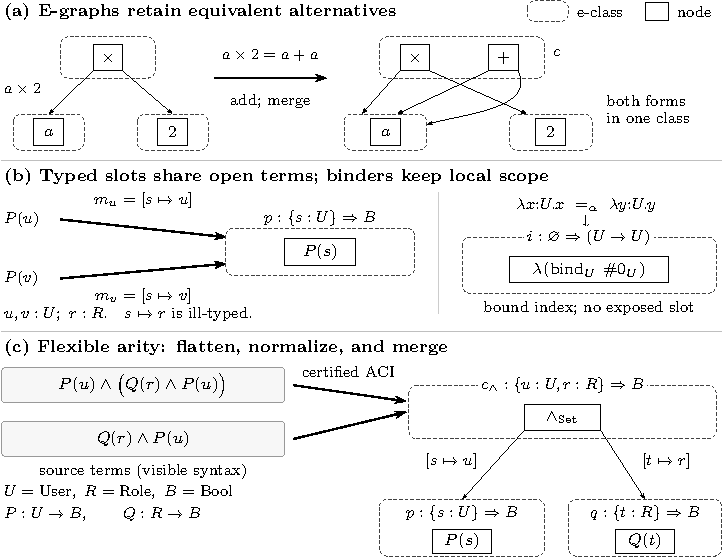
\includegraphics[width=\linewidth]{figures/typed-slotted-egraph-figure.pdf}
  \caption{E-graphs, typed slots, and flexible arity.
  (a) Rewriting retains equivalent alternatives.
  (b) Typed maps share shapes without equating distinct free invocations;
  bound indices stay local.
  (c) Certified associativity flattens visible syntax; the Set quotient removes
  order and duplicates. Dashed boxes are e-classes; solid inner boxes are e-nodes.}
  \label{fig:typed-slotted-egraphs}
\end{figure}


This propagation from equal children to equal parent expressions is called 
\emph{congruence}. %\Fix{Is it more appropriate to say ``To implement this, one uses...''?}
An implementation of it uses union--find to track merged
classes and \emph{hash-consing} to reuse nodes with the same operator and
child-class key. After a merge, a \emph{rebuilding} protocol updates parent keys and
merges any newly identical parents. To achieve \emph{equality saturation,} the
equation application and rebuilding process is repeated until no new nodes or equalities are found or a
resource limit is reached. The alternatives remain available until
\emph{extraction} selects a represented term, for example one with least
cost under a chosen cost model. In this paper, the e-graph provides the
shared structure on which flexible-arity operators and typed slot renamings
are combined.

\paragraph{Algebraic structure and binding.}
Ordinary positional nodes do not internalize associativity, commutativity,
and idempotence (ACI): explicit bidirectional rules may materialize many
parenthesizations and permutations. For conjunction, associativity permits
flattening nested conjunctions, commutativity forgets operand order, and
idempotence removes repeated operands. These are distinct choices: a
sequence preserves order and multiplicity, a bag forgets order but retains
multiplicity, and a set forgets both. Rewriting modulo AC and canonized
completion provides the established basis for flat bags and
sets~\cite{conchon2012canonized,kapur2021ModularAC}. Here we combine these
techniques with typed open-term interfaces.

Variable binding introduces a separate source of syntactic variation:
$\forall x{:}T.\,P(x)$ and $\forall y{:}T.\,P(y)$ differ only in a
consistently renamed bound variable. This is $\alpha$-equivalence, as a typed example is
shown in Figure~\ref{fig:typed-slotted-egraphs}(b). An open
term, such as the body $P(x)$ considered outside its quantifier, must retain
its dependence on $x$; sharing it in another scope therefore requires an
explicit account of which variable fills that position.

Prior work addresses these representation choices in several ways.
Egglog supports typed container values in a relational fixpoint
system~\cite{egglog,egglog_software}; E-graphs Modulo Theories supplies a
general interface to theory-specific canonical
domains~\cite{zucker2025omeletsneedonionsegraphs}. Lifting E-Graphs represents open
terms as functions over interfaces~\cite{zucker2026lifting}, while
Categorical E-Graphs treat binding through hierarchical
hypergraphs~\cite{egBindings}. Slotted E-Graphs instead expose a finite slot interface
$S_a$ for each class and represent an occurrence as $m*a$, where $m$ maps
$S_a$ into the caller~\cite{slottedEGraphs}. The slots record the class's
exposed variable positions; the map says which caller variables fill them.
%\Fix{I like the following explanation, but it is before the example is introduced. Although the example appears right after, we may want a sentence to frame that this is out typed setting via Alloy or to move it to an additional paragraph framing in the Alloy subsection.} 
Given a formal context with two defined types, \texttt{User} and \texttt{Photo}, 
there could be an arbitrary number of slots $u_1,...,u_k\in\texttt{User}, p_1,...,p_r\in\texttt{Photo}$
defined; 
in our typed setting, a \texttt{User} slot must map to a \texttt{User}
coordinate, and a \texttt{Photo} slot to a \texttt{Photo} coordinate.
The notation $m*a$ denotes an occurrence with that interface map, not a
claim that arbitrary assignments to its free variables give equal values.
Shapes quotient concrete slot
names; separately justified groups record symmetries, and a coordinate may be
removed only after independence is proved. De Bruijn indices normalize
ordinary alpha-renaming but do not express side-conditioned
permutations of declaration blocks~\cite{deBruijn,maziarz2021HashingAlpha}.

\paragraph{Alloy models and checks.}
Alloy is a typed relational specification language with temporal
operators~\cite{alloy,kodkod}. A model describes sets of objects and relations
between them. A \texttt{sig} declares a set of atoms, a field declares a
relation, \texttt{extends} declares a subsignature, and a \texttt{pred}
packages a formula. In the social-media model of
Figure~\ref{fig:alloy-certificate-example}, \texttt{User} and \texttt{Photo}
are sets, \texttt{Ad} is a subset of \texttt{Photo}, and
\texttt{follows: set User} associates each user with any number of users.
The multiplicity \texttt{one} in \texttt{date: one Day} requires exactly
one day per photo. Dot denotes relational join:
\texttt{u.follows.posts} is the set of photos posted by users whom
\texttt{u} follows. The formula \texttt{p in u.sees} tests whether
\texttt{u} sees \texttt{p}, and \texttt{all u: User |} universally
quantifies a user.

The Alloy Analyzer searches for instances satisfying a predicate with
\texttt{run}, or for counterexamples to an assertion with \texttt{check}.
The search uses a specified object scope and, for bounded temporal analysis,
trace bounds. Checking equivalence asks whether the two predicates can
disagree in a permitted instance; finding no disagreement is evidence within
those bounds. In our dataset, each exercise supplies an oracle predicate
expressing the intended constraint. A student predicate is overconstrained
when it excludes oracle-allowed instances, underconstrained when it admits
oracle-forbidden instances, or both. The evaluation inherits the dataset's
labels and reports its own bounded checks separately.

\paragraph{Scope of the construction.}
Our scope is the following composition: operator-declared
$\Seq/\Bag/\Set$ ports contain typed slot-mapped invocations, and their keys
are rebuilt jointly with leaders, invocation embeddings, certified slot
symmetries, and binder-block automorphisms. A port is an operator's declared
argument position or argument container. Flat construction opens only
visible applications of the same type-instantiated operator; it never unfolds
an opaque invocation. A carrier annotation contributes no semantic equation
without its endpoint-indexed certificate: the evidence must identify the
exact two well-typed expressions that the step equates.

In the Alloy study, \emph{canonical} means canonical under the implementation's
stored keys and declared rewrite vocabulary; the checked normal-form result
is instead generic over a supplied finite presentation. Neither layer claims
semantic completeness, unrestricted saturation termination, parser
correctness, full Java refinement, or full-corpus experimental replay.
